\section{Sharing Data Packages} \label{sec:sharing}

Because Morpho seamlessly connects to a network, you can easily share
your data packages with colleagues and/or view and open data packages
created by other scientists. After you have created a data package on
your local system, upload it to the network to share it with other users
(you control which users can view your data package via access
permissions). If other users have granted you permission to view their
data packages, you can also download data packages from the network and
open them on your computer.

By default, Morpho will share data packages on the KNB Metacat network.
If you wish to share data packages on another Metacat network, you must
specify the Metacat URL under \hyperref[sec:preferences]{Morpho
Preferences}. To open the Preference screen and change the network
(\autoref{fig:dialog-preferences}), select ``Set preferences'' from the
File menu.

\subsection{Uploading Data Packages to a Network} \label{sec:uploading}

After creating a data package and setting the Metacat URL (under File
$>$ Preferences), place the data package on the network in one of two
ways: by saving the data package or by synchronizing it. Use Save to
save the package to the local machine and/or the network. Use
synchronize to compare an existing data package on your local system to
those on the network and upload or download the package (if the versions
differ), ensuring that the local and network copies are identical. For
example, if you have made local changes that have not been saved to the
network (i.e., the local copy is more recent), then Synchronize will
transfer the local copy to the network. If a document was updated on
another computer (i.e., the network copy is more recent), then
Synchronize will copy the network version to your local machine.

To save a package to the network using the Save item in the File menu,
select the menu item and then choose whether to save the package
locally, on the network, or both (\autoref{fig:dialog-save-dp}).  Check
``Save to Network'' (or both ``Save to Network'' and ``Save Locally'')
and click ``Save''. If the data package is in EML 2.0.1 or earlier, you
will also see an option to ``Upgrade to latest EML (eml-2.1.0).'' 

\begin{figure}
  \centering
    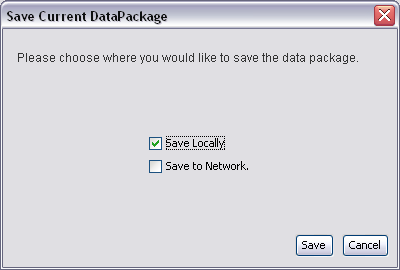
\includegraphics[width=0.7\textwidth]{images/dialog-save-dp.png}
  \caption{Select the location(s) to which to save the data package.}
  \label{fig:dialog-save-dp}
\end{figure}

\begin{shaded}
  \textbf{NOTE} Morpho automatically displays data packages stored in
  earlier versions of EML (e.g., 2.0 or Beta 6) as EML 2.0. If a package
  does not use the latest EML format, Morpho will prompt users to
  transform the EML to the latest version. If you choose to transform
  the EML, you must save the data package to preserve the changes, at
  which time the revision number of the document will be incremented. If
  the updated EML document is invalid (e.g., a required metadata field
  is blank), a correction wizard opens to allow users to fix the
  problem. For more information, please see \autoref{sec:upgrading-eml}.
\end{shaded}
 
To synchronize your data package, select ``Synchronize'' from the File
menu and then click the Execute button
(\autoref{fig:dialog-synchronize}). If you have made changes to the
local version of a package, the synchronize action will copy the local
package to the network, ensuring that the remote and local versions are
identical. If a package was updated on another computer (i.e., the
network copy is more recent), then Synchronize will copy the network
version to your local machine. Note that you cannot synchronize an
unsaved package.

\begin{figure}
  \centering
    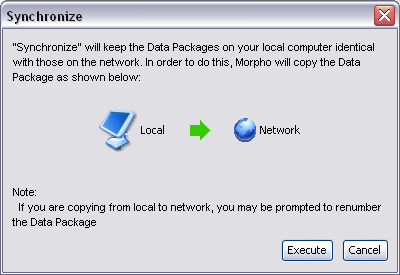
\includegraphics[width=0.7\textwidth]{images/dialog-synchronize.png}
  \caption{Synchronizing a data package.}
  \label{fig:dialog-synchronize}
\end{figure}

\subsection{Downloading Data Packages from a Network}

Users can download packages from a network to view and edit in Morpho
(in which case synchronization should be used) or to open with a local
application such as Excel (in which case an export should be used). To
download a data package from the network:
\begin{enumerate}
  \item From the \nameref{sec:panel-work} panel on the main Morpho
    screen, select ``Open an existing data package\ldots'' (to access
    your data package library) or ''Search for an existing data
    package\ldots'' (to access packages created by other users). 
  \item Select a data package and right-click to reveal a drop-down
    action menu (\autoref{fig:search-results-download}). Select the
    Synchronize menu item. Note: You can also choose to synchronize from
    the File menu.
  \item Morpho will copy the selected data package to your local system,
    ensuring that the local and network copies are identical.
\end{enumerate}

\begin{figure}
  \centering
    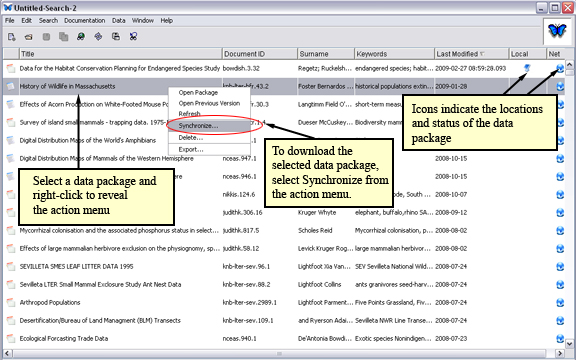
\includegraphics[width=0.7\textwidth]{images/search-results-download.jpg}
  \caption{To download a data package, choose synchronize from the
    right-click menu.}
  \label{fig:search-results-download}
\end{figure}

\subsection{Exporting Data Packages }

To save a data package for use outside Morpho (such as with Excel),
choose to Export the package. To export a package, follow the steps for
synchronizing, except choose Export from the drop-down action menu. You
can export to a directory or to a .zip file, which will allow you to
easily transport the package. If you choose to export to a directory,
you will be prompted to select a directory
(\autoref{fig:dialog-export-package}).

\begin{figure}
  \centering
    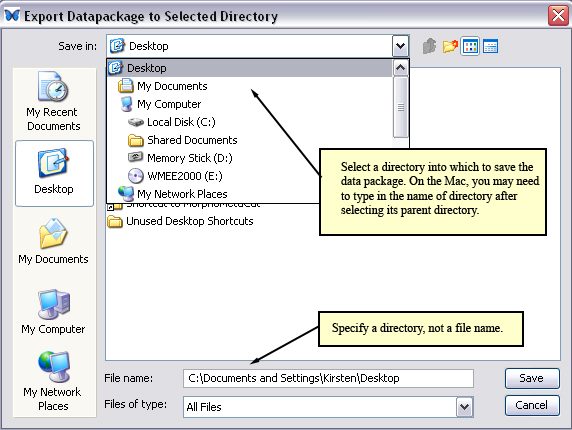
\includegraphics[width=0.7\textwidth]{images/dialog-export-package.jpg}
  \caption{Exporting a data package to a directory. Select a directory.}
  \label{fig:dialog-export-package}
\end{figure}

Note that you must specify a directory, not a file. Select a directory
into which to export the package. On the Mac, you may need to type the
name of directory after selecting its parent directory. The exported
metadata and data (if your data package includes data) will be exported
to the specified directory.

EML data packages can be exported as different metadata language
standards (\autoref{fig:dialog-export-metadata}). Currently Morpho can
produce files in the Biological Data Profile format.

\begin{figure}
  \centering
    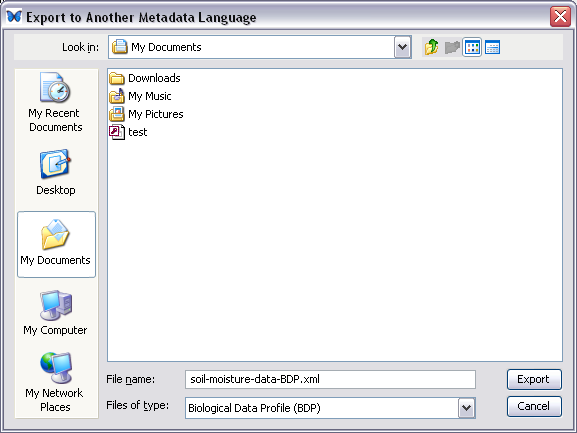
\includegraphics[width=0.7\textwidth]{images/dialog-export-metadata.png}
  \caption{Exporting a data package to another metadata format.}
  \label{fig:dialog-export-metadata}
\end{figure}

\subsection{Importing an EML file as a new Data Package}
\label{sec:importing}

EML files on the local file system can be imported into Morpho as a new
data package (\autoref{fig:dialog-import-metadata}). The data package
can then be saved to network for sharing. Select the “Import” menu item
from the File menu to start the import process.

\begin{figure}
  \centering
    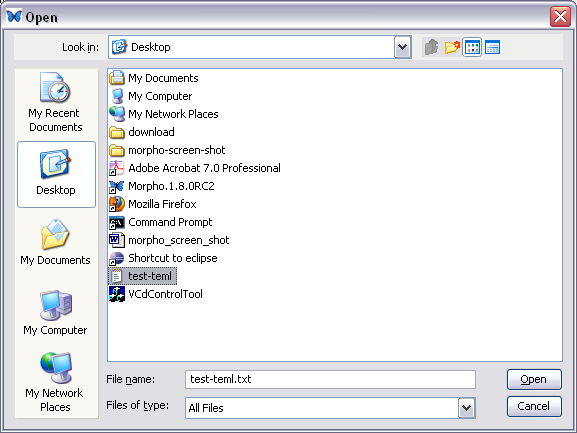
\includegraphics[width=0.7\textwidth]{images/dialog-import-metadata.png}
  \caption{Importing an EML file into Morpho as a Data Package.}
  \label{fig:dialog-import-metadata}
\end{figure}
